\chapter{les \textit{wearable devices} au sein des habitats intelligents}
\label{chap:3}

\section{Introduction}

Dans le chapitre précédent, le processus d'apprentissage pour la reconnaissance d'activités a été présenté dans un cas d'application générique. De nombreuses étapes, depuis l'obtention des données brutes jusqu'à la classification des activités à reconnaître, y ont été détaillées. Néanmoins, dans un contexte d'utilisation avec des \textit{wearable devices}, la manière dont ces données sont acquises n'a, quant à elle, pas été mentionnée. De plus, l'adaptation de ce processus avec ces dispositifs fait intervenir une étape supplémentaire de transmission des données. Ce chapitre commence par définir la notion de \textit{wearable devices}, puis il traite plus en détail des composants matériels et logiciels qui sont plus spécifiques dans l'utilisation de ces dispositifs au sein des habitats intelligents.

\section{Définitions}

Selon le rapport publié par l'\cite{InternationalTelecommunicationUnion2012}, l'internet des objets (\acl{IoT} ou \acs{IoT}) représente une \og infrastructure mondiale pour la société de l'information, qui permet de disposer de services évolués en interconnectant des objets (physiques ou virtuels) grâce aux technologies de l'information et de la communication interopérables existantes ou en évolution \fg. Ainsi, d'un point de vue conceptuel, l'\acs{IoT} caractérise des objets physiques connectés ayant leur propre identité numérique et la capacité de communiquer les uns avec les autres. Ce réseau crée, en quelque sorte, une passerelle entre le monde physique et le monde virtuel. En d'autres termes, il s'agit de fournir une identification numérique directe et normalisée (adresse IP, protocoles de communication, \textit{etc.}) d'un objet physique grâce à un système de communication sans-fil qui peut être du Bluetooth ou encore du Wi-Fi.

Par conséquent, les \textit{wearable devices} appartiennent aux objets connectés, puisqu'ils se caractérisent plus particulièrement comme une technologie qui embarque des capteurs et qui est disposée directement sur le corps humain. \cite{Godfrey2018} ont identifié deux types de \textit{wearable devices} : les dispositifs autonomes (\textit{p. ex.} les moniteurs d'activités physiques) et les dispositifs de mesure (\textit{p. ex.} un moniteur de fréquence cardiaque porté sur la poitrine). Les dispositifs autonomes permettent de réaliser différents traitements, plus ou moins complexes, dont les résultats sont ensuite communiqués à d'autres appareils, tandis que les dispositifs de mesure ont, quant à eux, pour seul objectif de transférer les informations du capteur vers un serveur, par exemple.

Les principaux avantages offerts par les \textit{wearable devices}, comme leur taille, leur faible prix ou leur facilité d'utilisation, ont favorisé leur usage dans différents domaines de recherche tels que la surveillance des activités physiques et sportives, la surveillance en continu de la santé ou encore la reconnaissance de gestes, d'activités ou de chutes. \citep{Seon-WooLee2002, Istepanian2011, Garcia-Ceja2014, Bayat2014, YuanJieFan2014, Gao2014, Nielsen2014, Adib2015, Davis2016, Khan2016, Chapron2018}.

\section{Les capteurs}

Pour réaliser le processus d'apprentissage permettant de mettre en place une reconnaissance, la première étape consiste à récolter des données brutes qui sont produites par des capteurs. Cependant, puisqu'il en existe une grande diversité, il semble nécessaire d'identifier ceux qui sont les plus adéquats pour être proposés en tant que \textit{wearable devices}. Pour ce faire, cette section présente, en ce basant sur la taxonomie d'\cite{Acampora2013}, les capteurs parmi ceux qui sont les plus utilisés dans ce domaine d'application.

\subsection{Les capteurs de mouvements}

Les centrales inertielles (\aclp{IMU} ou \acsp{IMU}) sont les capteurs de mouvement qui sont le plus fréquemment implantés dans les \textit{wearable devices} de par leur simplicité d'utilisation. Celles-ci peuvent comporter d'un à trois types de capteurs différents : les accéléromètres, les gyroscopes et les magnétomètres. Ils permettent de mesurer respectivement l'accélération linéaire, la vitesse angulaire et l'intensité du champ magnétique que subissent les objets auxquels ils sont fixés, grâce à un maximum de trois axes orthogonaux ($x,\: y\: $ et $\: z$). L'adoption de ces capteurs a permis de nombreuses applications concrètes, telles que la reconnaissance de chutes chez les personnes âgées, l'identification de l'orientation du corps, la réadaptation, ainsi que la reconnaissance d'activités quotidiennes \citep{Seon-WooLee2002, Garcia-Ceja2014, Bayat2014, Gao2014, Davis2016, Chapron2018}.

\subsection{Les capteurs physiologiques}

Grâce aux progrès technologiques et plus particulièrement à la miniaturisation de l'électronique, de nouveaux types de capteurs, jusqu'alors réservés au domaine médical, ont pu être utilisés pour récolter les données physiologiques des utilisateurs, sans pour autant recourir aux services spécialisés d'un hôpital. Cependant, certaines techniques sont encore considérées comme complexes et intrusives à la fois. C'est, par exemple, le cas de l'\ac{EEG} qui demeure encore rarement exploité. Ce capteur physiologique permet d'obtenir la représentation de l'activité électrique du cerveau par l'intermédiaire d'électrodes disposées sur le crâne d'un individu. Néanmoins, plusieurs autres capteurs physiologiques ont, quant à eux, été très largement utilisés, et ce, dans de nombreux domaines de recherche. Parmi ceux-ci, il est possible de mentionner les capteurs qui permettent l'acquisition de l'\ac{ECG}, c'est-à-dire, la représentation graphique de l'activité électrique du c\oe{}ur ; de l'\ac{EMG}, soit l'activité électrique produite par les muscles ; de capteurs mesurant la glycémie, qui indique le taux de concentration de glucose dans le sang, ou de la \ac{SPO2}, qui désigne le taux de saturation du sang en oxygène. Au sein des habitats intelligents, l'intégration de ces capteurs dans des \textit{wearable devices} a principalement permis de proposer de nouvelles techniques pour la réhabilitation \citep{YuanJieFan2014}, la reconnaissance de gestes \citep{Jung2015, Benatti2015, Tavakoli2018} et la surveillance en continu de la santé des résidents pour détecter de possibles maladies \citep{Istepanian2011, Adib2015, Khan2016}.

\subsection{Les capteurs de courbure et de force}

\begin{figure}[b!]
    \centering
	\subfloat[Capteur de courbure]{
		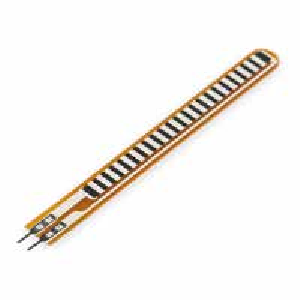
\includegraphics[width=.35\linewidth]{chapter3/flex_sensor.pdf}
		\label{fig:flex_sensor}
    }
    \hspace*{2cm}
	\subfloat[Capteur de force (\acs{FSR})]{
		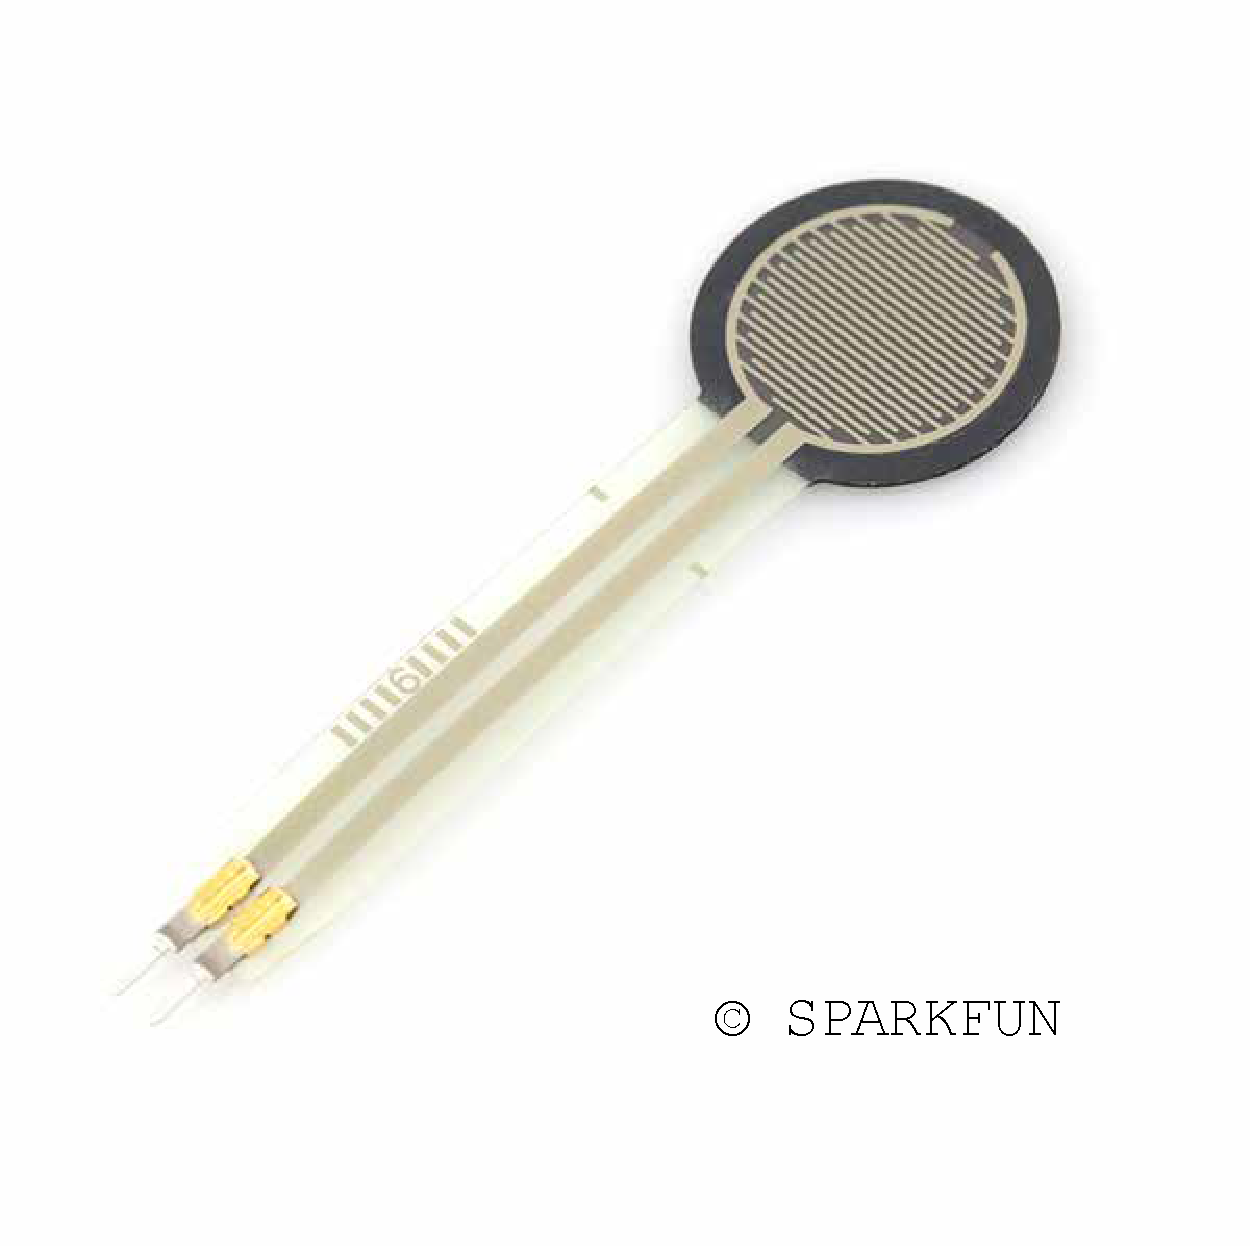
\includegraphics[width=.35\linewidth]{chapter3/force_sensor.pdf}
		\label{fig:force_sensor}
    }
    \caption{Exemples de capteurs de courbure (a) et de force (b).}
    \label{fig:flex_force_sensors}
\end{figure}

Certains dispositifs considérés comme des \textit{wearable devices} tels que les gants présentés par \cite{Sanford2015} et \cite{Zheng2016} ainsi que les chaussures conçues par \cite{Bamberg2008} et \cite{Bae2013}, ont nécessité l'utilisation de capteurs de courbure (\textit{flex sensors}) et de force (\aclp{FSR} ou \acsp{FSR}). Ces capteurs, respectivement montrés en figures \ref{fig:flex_sensor} et \ref{fig:force_sensor} fonctionnent grâce à des résistances dont la valeur change respectivement en fonction de la courbe qui est donnée au capteur ou de la pression qui est appliquée sur la surface de contact. Ainsi, comme illustré par ces différentes recherches, ces capteurs se sont montrés utiles dans certaines applications de réadaptation et de reconnaissance de gestes et d'activités.

\subsection{Les capteurs environnementaux}

Les capteurs environnementaux comportent principalement les capteurs de pression barométrique, d'humidité, de température et de dioxyde de carbone (CO\textsubscript2). Ils sont principalement utilisés pour fournir des informations relatives à l'environnement proche des utilisateurs de \textit{wearable devices}. Ainsi, les données produites par ce type de capteur peuvent être utilisées pour identifier le contexte d'utilisation dans lequel leurs porteurs évoluent et par conséquent, renforcer les analyses réalisées grâce aux autres capteurs \citep{Acampora2013}. Par ailleurs, certains capteurs d'humidité et de température ont également été utilisés pour fournir des informations nécessaires à la surveillance de l'état de santé des utilisateurs des \textit{wearable devices} \citep{Anliker2004}.

\section{Les technologies de communication sans-fil}

Lorsqu'il est appliqué à des \textit{wearable devices}, le processus d'apprentissage nécessite une étape supplémentaire qui est la transmission de données. Ces dernières peuvent être les données brutes, les caractéristiques ou les décisions qui sont émises en sortie de l'algorithme d'apprentissage. En fonction des cas et des capteurs que peut comporter le dispositif, la fréquence d'émission ainsi que le poids des données à transmettre peut fortement varier. Ainsi, il est nécessaire de choisir une technologie de communication sans-fil adéquate pour chaque situation. Cette section va donc s'intéresser à celles qui sont les plus communément utilisées par les \textit{wearable devices} existants.

\subsection{Les topologies des réseaux}
\label{sec:topo}

Avant d'entrer dans le détail des technologies de communication utilisées par les \textit{wearable devices}, il est important de commencer par énoncer les topologies de réseaux existantes dans le domaine du sans-fil. En effet, elles jouent un rôle important dans le bon fonctionnement de la communication réseau et l'identification de leur différentes caractéristiques va permettre, \textit{a posteriori}, de mieux cibler les besoins pour le développement de nouveaux systèmes. D'après \cite{Tanenbaum2011}, les topologies les plus fréquemment mises en place dans un contexte sans-fil sont :

\begin{itemize}[label=\textbullet]
	\item
	      La \textbf{diffusion (\textit{broadcast})} (figure \ref{fig:topo_broadcast}) où un message est envoyé par un n\oe{}ud émetteur à tous les n\oe{}uds récepteurs du réseau qui sont à sa portée. Le canal de communication est unidirectionnel et aucun accusé de réception n'est transmis au n\oe{}ud émetteur depuis les n\oe{}uds récepteurs.
	\item
          Les \textbf{réseaux en étoile} (figure \ref{fig:topo_star}) admettent un n\oe{}ud émetteur-récepteur central qui communique, à travers plusieurs canaux bidirectionnels, avec plusieurs autres n\oe{}uds émetteurs-récepteurs périphériques. Ces émetteurs-récepteurs périphériques ne peuvent pas communiquer directement les uns avec les autres.
    \item
        Les \textbf{réseaux pair-à-pair (\acl{P2P} ou \acs{P2P})} permettent à deux n\oe{}uds émet\-teurs-récepteurs, reliés par un canal de communication bidirectionnel, d'échanger des données dans les deux sens, tel qu'illustré par la figure \ref{fig:topo_p2p}.
    \item
        Les \textbf{réseaux maillés} (figure \ref{fig:topo_mesh}) permettent l'échange de données entre n'importe quels n\oe{}uds du réseau sans passer par un n\oe{}ud central. La communication est bidirectionnelle et chaque n\oe{}ud peut-être relié à plusieurs autres n\oe{}ud qui composent le réseau.
    \item
        Le \textbf{mode scan} (figure \ref{fig:topo_scan}) permet à un n\oe{}ud central de fonctionner en mode réception, c'est-à-dire, en attente de recevoir un signal provenant de n'importe quel n\oe{}ud émetteur qui est à sa portée. La communication entre les deux n\oe{}uds est unidirectionnelle et se fait du n\oe{}ud émetteur vers le n\oe{}ud central.
\end{itemize}

\begin{figure}[H]
    \centering
    \subfloat[Diffusion]{
        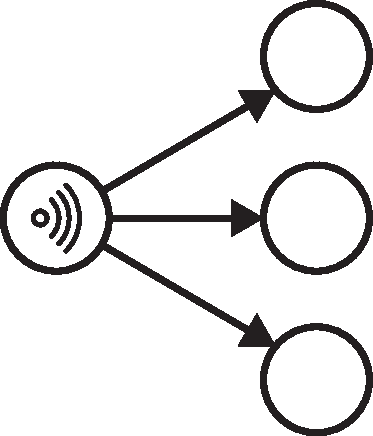
\includegraphics[width=.2\linewidth]{chapter3/topo_broadcast.pdf}
        \label{fig:topo_broadcast}
    }
    \hspace*{.2\linewidth}
    \subfloat[Étoile]{
        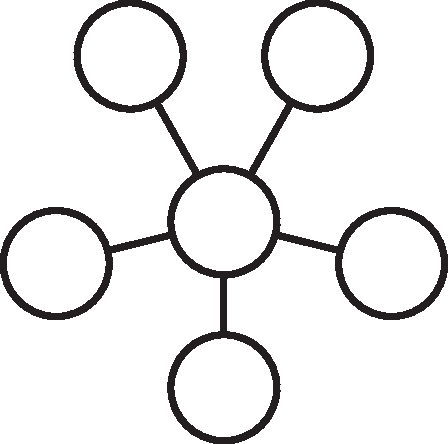
\includegraphics[width=.22\linewidth]{chapter3/topo_star.pdf}
        \label{fig:topo_star}
    }
    \\[30pt]
    \subfloat[Pair-à-Pair]{
		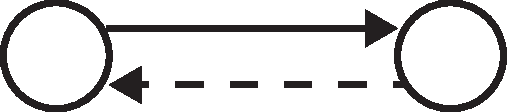
\includegraphics[width=.3\linewidth]{chapter3/topo_p2p.pdf}
		\label{fig:topo_p2p}
    }
    \hspace*{.1\linewidth}
	\subfloat[Maillé]{
		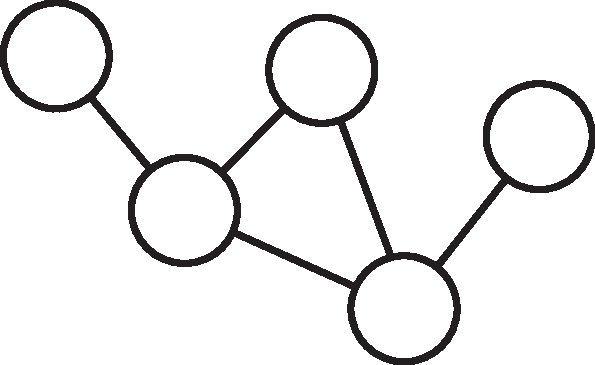
\includegraphics[width=.3\linewidth]{chapter3/topo_mesh.pdf}
		\label{fig:topo_mesh}
    }
    \\[30pt]
    \subfloat[Mode scan]{
		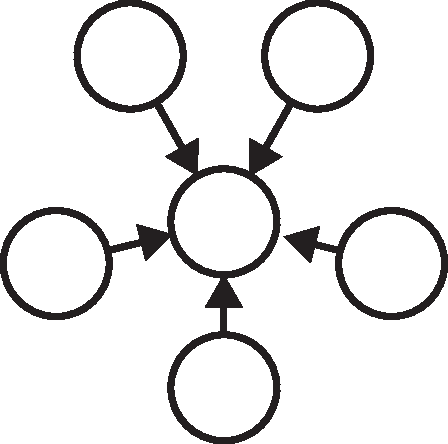
\includegraphics[width=.22\linewidth]{chapter3/topo_scan.pdf}
		\label{fig:topo_scan}
    }
	\caption{Représentation des topologies réseaux pour les technologies de communication sans-fil.}
\end{figure}

\subsection{Wi-Fi}
Le Wi-Fi, régi par le standard IEEE 802.11\footnote{\url{https://goo.gl/X9WKyx}}, est probablement la technologie de communication sans-fil la plus connue, car nous l'utilisons massivement depuis deux décennies. En constante amélioration, chaque génération du standard a apporté aussi bien des vitesses plus rapides et une latence réduite, qu'une meilleure expérience utilisateur dans une multitude d’environnements et avec divers types de périphériques. Toutes utilisations confondues, le standard qui est actuellement le plus utilisé est le Wi-Fi 802.11ac. Bien qu'il offre des vitesses de transfert de données à haut débit (de 400 Mbit/s à 2.6 Gbit/s), sa portée reste dans la moyenne de celles proposées par d'autres technologies, soit plusieurs dizaines de mètres. Néanmoins, dans le contexte des \textit{werable devices}, le standard 802.11n sur la bande de Fréquence 2.4GHz, qui est le plus utilisé. Bien que celui-ci permette d'obtenir une portée plus élevée de quelques dizaines de mètres, les  vitesses de transfert de données demeurent plus faibles (de 72 à 288 Mbit/s). Par ailleurs, le plus gros inconvénient de cette technologie reste sa forte consommation énergétique, ce qui est un facteur extrêmement limitant pour les objets connectés (\acs{IoT}), parmi lesquels se retrouvent les \textit{wearable devices}.

Dans un futur proche, les évolutions prévues dans les standards 802.11ah et 802.11ax vont principalement se concentrer sur l'amélioration de la consommation énergétique afin que l'utilisation du Wi-Fi devienne adaptée pour l'\acs{IoT}. Néanmoins, la contrepartie de cette évolution est l'impact sur la vitesse de transfert de données, qui va alors, devenir beaucoup plus faible (8 Mbit/s) \citep{Sun2013}.

\subsection{Bluetooth Low Energy (\acs{BLE})}
\label{subec:com_ble}

Le \acs{BLE}\footnote{\url{https://www.bluetooth.com/specifications}} a été lancé en 2010 dans le cadre de la spécification du Bluetooth 4.0. Bien souvent, il est considéré comme une version plus légère et plus optimisée du Bluetooth classique (versions 1 à 3), mais en réalité, le \acs{BLE} présente une conception totalement différente. En effet, ce dernier a été pensé pour être une technologie de communication proposant une consommation d'énergie très faible, spécifiquement optimisée pour pouvoir offrir un coût réduit, une faible bande passante, ainsi qu'une complexité moindre. En comparaison aux autres technologies de communication sans-fil à faible consommation, le \acs{BLE} a connu une adoption très rapide principalement grâce à la croissance phénoménale des téléphones intelligents et plus généralement de l'informatique mobile. Ainsi, les leaders de l’industrie mobile comme Apple ou Samsung ont favorisé le large déploiement de cette technologie qui est aujourd'hui, la technologie de communication la plus utilisée par les \textit{wearable devices} \citep{Gomez2012}.

D'autre part, avec l'arrivée des premiers appareils supportant la version 5 du Bluetooth, cette technologie devient la seule à supporter, intuitivement, l'intégralité des topologies réseaux présentées dans la sous-section \ref{sec:topo}. En effet, en plus d'offrir un débit et une portée deux fois supérieurs à celui de la quatrième version, soit 2 Mbit/s et 250 mètres respectivement, cette nouvelle spécification intègre également la nouvelle norme : \og Bluetooth Mesh 1.0 \fg, qui va permettre la mise en place d'un réseau maillé\footnote{\url{https://www.bluetooth.com/specifications/mesh-specifications}}. Cependant, il ne sera pas possible de tirer profit de tous ces nouveaux avantages en même temps, puisque cette cinquième version permettra deux modes de fonctionnement : haut débit ou longue portée. Ainsi, dans le premier cas, la vitesse de transfert sera favorisée au profit de la portée et inversement, ceci dans le but de continuer les efforts pour la réduction de la consommation d'énergie tout en améliorant les capacités.

\subsection{ZigBee}
\label{subec:com_zigbee}

La technologie ZigBee a été développée dans les années 1990 et avec l'avènement des objets connectés, elle est devenue l'une des technologies de communication parmi les plus utilisées. En comparaison avec le Wi-Fi, le ZigBee admet l'avantage de ne consommer que peu d'énergie. De plus, le standard IEEE 802.15.4\footnote{\url{https://goo.gl/X9WKyx}}, qui régit cette technologie, indique que le ZigBee peut offrir une porté de plusieurs kilomètres, en fonction de la puissance de l'émetteur et de certaines caractéristiques environnementales.

Initialement, le ZigBee a été introduit pour répondre à des problématiques liées à l'hétérogénéité de l'\acs{IoT} \citep{Rahmani2015, Cho2013} et par extension, des technologies présentes au sein des habitats intelligents \citep{Hui2017}. ZigBee permet de s'appuyer sur la conception d'une topologie de réseau maillé (\textit{mesh}). De ce fait, certains \textit{wearable devices} \citep{Cruz2018} et habitats intelligents \citep{Cook2013} ont vite adopté cette technologie, ce qui a, par exemple, permis à \cite{Cook2013}, d'unifier et de simplifier la communication entre tous les capteurs présents dans l'habitat CASAS.

\subsection{La Communication en Champ Proche}

La communication en champ proche (\acl{NFC} ou \acs{NFC}) est une technologie de communication sans-fil à faible consommation et de courte portée, permettant l'échange d'informations entre des périphériques jusqu'à une distance de l'ordre du centimètre. L'avantage principal de cette technologie est que les périphériques \acs{NFC} passifs, par exemple, les cartes de crédit, ne requièrent aucune alimentation. Ils deviennent actifs uniquement lorsqu'ils entrent dans le champ proche d'un périphérique qui est alimenté (\textit{p. ex.} un lecteur).

Cette technologie de communication s'est principalement popularisée grâce aux méthodes de paiement sans contact \citep{Ondrus2007}, mais elle a également été utilisée dans plusieurs recherches relatives aux environnements intelligents. Par exemple, \cite{Pering2007} ont proposé un système de reconnaissance de gestes qui exploite le \acs{NFC} d'un téléphone intelligent. Aussi, \cite{Chang2009} ont proposé une architecture pour l'automatisation du contrôle des installations électriques d'une maison, grâce à un système de reconnaissance d'utilisateurs de téléphones intelligents qui s'appuie principalement sur une détection d'appareils \acs{NFC} présents dans l'environnement.

La limitation de cette technologie en termes de distance ne fait pas du \acs{NFC} un concurrent direct du \acs{BLE} ou du ZigBee. Son adoption concerne plutôt un marché de niche et il est préférable de le considérer comme complémentaire aux autres technologies de communication sans-fil présentées dans ce chapitre.

\subsection{Bilan des technologies de communication sans-fil}

\begin{table}[b!]
    \caption{Caractéristiques des différentes technologies de communication sans-fil employées par les \textit{wearable devices}}
    \label{tab:wireless_tech}
    \resizebox{\columnwidth}{!}{
        \begin{tabular}{c|c|c|c|c|c|}
            \cline{2-6}
            \multicolumn{1}{l|}{} & \textbf{Portée} & \textbf{Débit} & \textbf{Latence} & \textbf{\begin{tabular}[c]{@{}c@{}}Pic de\\[-15pt] consommation\end{tabular}} & \textbf{\begin{tabular}[c]{@{}c@{}}Consommation\\[-15pt] moyenne\end{tabular}} \\ \hline
            \multicolumn{1}{|c|}{\textbf{\begin{tabular}[c]{@{}c@{}}Wi-Fi\\[-15pt] (812.11n)\end{tabular}}} & 70 m & 150 - 600 MB/s & $O(1\: ms)$ & 150 mA & 100 mA \\ \hline
            \multicolumn{1}{|c|}{\textbf{\begin{tabular}[c]{@{}c@{}}Wi-Fi\\[-15pt] (812.11ac)\end{tabular}}} & 35 m & 433 - 2600 MB/s & $O(1\: ms)$ & 150 mA & 100 mA \\ \hline
            \multicolumn{1}{|c|}{\textbf{BLE}} & 250 m & 1 - 2 MB/s & $O(1\: ms)$ & 15 mA & 25 $\mu$A \\ \hline
            \multicolumn{1}{|c|}{\textbf{ZigBee}} & > 1 km & 250 kB/s & $O(1\: s)$ & 30 mA & 30 mA \\ \hline
            \multicolumn{1}{|c|}{\textbf{NFC}} & 0.1 m & 400 kB/s & $O(1\: s)$ & 50 mA & 50 mA \\ \hline
        \end{tabular}
    }
\end{table}

Dans cette section, les technologies de communications sans-fil les plus utilisées par les \textit{wearable devices} ont été présentées. Puisqu'elles admettent des caractéristiques différentes, il convient donc d'en proposer une synthèse. Pour ce faire, le tableau \ref{tab:wireless_tech} illustre les différences techniques pertinentes pour ces technologies. La consommation énergétique est identifiée, pour chacune d'elles, par les valeurs théoriques de la consommation moyenne ainsi que du pic de consommation, c'est-à-dire, la valeur maximum de l'intensité du courant. De plus, la latence théorique y est également proposée. Puisque cette dernière caractéristique permet de mesurer le temps nécessaire à la transmission d'un signal entre un émetteur et son récepteur, elle aura donc un impact significatif sur la consommation énergétique. En effet, une forte latence va permettre de consommer moins d'énergie et inversement dans le cas d'une latence faible.

Dans le vaste monde des technologies sans-fil et plus particulièrement celles à faible consommation d'énergie, seules quelques-unes d'entres elles se sont popularisées avec le développement de l'\acs{IoT} et des \textit{wearable devices}. Parmi celles-ci, il est possible de retrouver le Wi-Fi, le \acs{BLE}, le ZigBee et le \acs{NFC}. Bien que chacune d'elles puisse être utilisée avec ces dispositifs ayant une autonomie de fonctionnement limitée, elles admettent des capacités de portée, de débit et de robustesse différentes. Ces variations de performances impliquent que chaque méthode de communication possède un cas d'application qui lui est propre. Le choix de la technologie à adopter dans le processus de conception de \textit{wearable devices} est donc crucial et doit être effectué rigoureusement en fonction de l'utilisation qui doit en être faite.

\section{Les échanges de données}

Dans la section précédente, les différentes technologies de communication sans-fil ont été présentées. Ces différentes technologies constituent la couche matérielle du modèle de communication réseau. Par conséquent, cette section s'intéresse plus en détail aux différents protocoles de communication appartenant, quant à eux, aux couches hautes de ce même modèle de communication et qui sont les plus utilisés dans le contexte des réseaux de capteurs sans-fil.

\subsection{Le modèle \textit{publish/subscribe}}

Depuis l'arrivée des habitats intelligents, certaines architectures comme celle proposée pour CASAS \citep{Cook2013} ont adopté le modèle \textit{publish/subscribe} pour l'ensemble de leurs réseaux de capteurs. Depuis, plusieurs travaux se sont principalement intéressés à l'utilisation de ce modèle pour l'intégration de l'\acs{IoT} au sein de ces habitats \citep{Lee2014, Upadhyay2016, VandenBossche2018}.

Le modèle \textit{publish/subscribe} est une alternative au modèle client/serveur traditionnel où un client communique directement avec le serveur. Dans se modèle, il est possible de distinguer deux types de clients : ceux qui envoient des messages, les \textit{publishers} et ceux qui les reçoivent, les \textit{subscribers}. Dans une vaste majorité des utilisations de ce modèle, les \textit{publishers} et les \textit{subscribers} n'échangent jamais directement et il ne savent pas que l'autre existe physiquement. Le lien entre eux est fait par l'intermédiaire d'un troisième composant, le \textit{broker}. Son rôle est de filter les messages entrant et de les redistribuer correctement aux différents \textit{subscribers} comme illustré par la figure \ref{fig:pub_sub}. L'avantage principal du modèle \textit{publish/subscribe} est son élasticité. En effet, il est assez simple de voir comment il est possible de paralléliser les opérations exécutées par le \textit{broker}. De plus, les messages peuvent être gérés comme des évènements qu'il ne restera alors qu'a intercepter.

\begin{figure}[H]
	\centering
	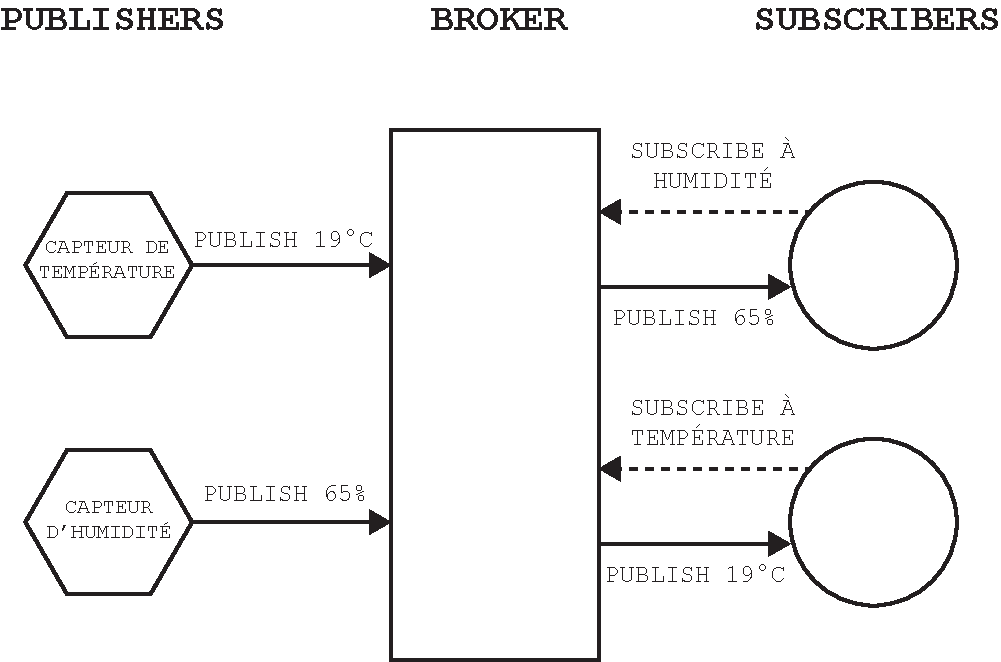
\includegraphics[width=10cm]{chapter3/pub_sub.pdf}
        \caption{Illustration du fonctionnement du modèle de communication de type \textit{publish/subscribe}.}
	\label{fig:pub_sub}
\end{figure}

Le modèle \textit{publish/subscribe} connaît de nombreuses implémentations parmi lesquelles il est possible de retrouver \ac{AMQP} \citep{Vinoski2006}, \ac{XMPP} \citep{Saint-Andre2011}, RabbitMQ \citep{Dossot2014} et ZéroMQ \citep{Hintjens2013}. Cependant, \ac{MQTT} est la plus connue d'entre elles \citep{Hunkeler2008}. En effet, grâce à sa portabilité \footnote{\url{https://github.com/mqtt/mqtt.github.io/wiki/libraries}} et sa faible consommation de ressources (débit, mémoire et consommation d'énergie), elle demeure une excellente solution pour l'échange de données dans le domaine de l'\acs{IoT}, où la puissance des dispositifs reste encore relativement limitée. En plus des avantages offerts par le modèle \textit{publish/subscribe}, \acs{MQTT} propose la définition de trois différents niveaux de qualité de service (\acl{QoS} ou \acs{QoS}) : Le message est distribué une fois tout au plus, ou n'est pas distribué du tout ; le message est toujours distribué au moins une fois ou le message est toujours distribué une seule fois. Ceux-ci permettent donc une plus grande flexibilité en ce qui concerne le niveau de fiabilité requis par le système ; c'est-à-dire, la garantie que les messages sont, ou non, correctement envoyés et reçus. Aussi, dans son objectif de demeurer une solution légère, \acs{MQTT} permet d'avoir recours à une option de sécurité relativement simple. Cette dernière consiste en une authentification des clients auprès du \textit{broker} \textit{via} un nom d'utilisateur et un mot de passe. Néanmoins, plusieurs couches de sécurité supplémentaires peuvent y être ajoutées (utilisation d'un réseau privé virtuel (\acl{VPN} ou \acs{VPN}) ou le chiffrement des échanges de messages par \acs{SSL}/\acs{TLS}, \textit{etc.})

\subsection{Le cas spécifique du \acs{BLE}}

D'après le rapport publié par \cite{ON2017}, le \ac{BLE} serait la technologie de communication sans-fil la plus utilisée dans le domaine de l'\acs{IoT} et plus particulièrement des \textit{wearable devices}. De ce fait, la sous-section \ref{subec:com_ble} ayant présenté les principales caractéristiques techniques de bas niveau pour cette technologie, il est désormais nécessaire d'en présenter le fonctionnement de haut niveau. En effet, la communication par \acs{BLE} oblige l'utilisation du protocole tel que défini par le standard. Par conséquent, l'implémentation d'un tout autre protocole de haut niveau déjà existant n'est pas possible avec cette technologie.

Le protocole du \acs{BLE} est divisé en deux catégories: le contrôleur et l'hôte ; chacune admettant des sous-catégories parmi lesquelles il est possible de retrouver le \ac{GAP} et le \ac{GATT}. Le \acs{GAP} définit la topologie générale du réseau. En d'autres termes, si un dispositif Bluetooth est visible par d'autres, c'est par l'intermédiaire de ce profil. Il détermine comment les appareils peuvent, ou non, interagir entre eux. Le \acs{GATT}, quant à lui, décrit en détail la manière dont les données sont formatées, conditionnées et transférées selon les règles définies par l'\ac{ATT}. Pour communiquer avec le monde extérieur, un appareil \acs{BLE} peut se trouver en deux modes différents : le mode diffusion (figure \ref{fig:topo_broadcast}) ou le mode communication, qui correspond à une topologie étoile (figure \ref{fig:topo_star}). Ceux-ci sont définis dans les directives relatives au \acs{GAP}.

Dans le cas du mode diffusion, il est important de distinguer deux rôles que peuvent avoir les appareils \acs{BLE} : les diffuseurs et les observateurs. Pendant un intervalle de temps donné (l'intervalle de diffusion), le diffuseur est responsable d'annoncer publiquement des données. Si un observateur demande à récupérer les données annoncées par le diffuseur, ce dernier doit alors lui transmettre\textemdash sinon elles sont annoncées de nouveau dès lors que l'intervalle de diffusion est écoulé. Un nouveau cycle peut alors recommencer. En outre, il est important de noter qu'aucune connexion n'est établie entre un observateur et un diffuseur. Le fonctionnement de ce processus est illustré par la figure \ref{fig:ble_broadcast_process}.

À l'inverse du mode diffusion, deux appareils \acs{BLE}, lorsqu'ils sont en mode communication, doivent explicitement établir une connexion entre eux pour que des données puissent être échangées. Si un observateur demande une connexion à un diffuseur, le processus de diffusion s'arrête et il n'est plus possible d'obtenir les données qui étaient annoncées. Ce dernier adopte alors le rôle de périphérique et l'observateur devient le central. Un appareil \acs{BLE} ayant le rôle de périphérique ne peut se connecter qu'à un seul dispositif central à la fois, mais un central peut, quant à lui, être connecté à plusieurs périphériques. Cependant, la connexion peut être interrompue intentionnellement ou non (\textit{p. ex.} perte de l'alimentation), et ce, par n'importe quel dispositif.

Dès que la connexion est établie, la communication entre le dispositif central et le dispositif périphérique peut commencer. Le dispositif qui demande les données joue alors le rôle de serveur \acs{GATT}. Puisque les rôles définis par le \acs{GAP} et le \acs{GATT} sont indépendants, le central et le périphérique peuvent tous deux devenir le serveur. Celui-ci est donc sollicité par le client \acs{GATT} qui lui envoie des requêtes. Le serveur \acs{GATT} indique un intervalle de connexion au client qui va alors essayer de se reconnecter après chaque délai pour récupérer de nouvelles données, si elles existent. Une représentation graphique du fonctionnement de ce processus est donnée en figure \ref{fig:ble_connect_process}. Les données sont transmises du serveur au client par une collection de services. Ceux-ci sont utilisés pour diviser les données en entités logiques et contiennent des blocs de données spécifiques qui sont les caractéristiques. Un service peut avoir une ou plusieurs caractéristiques et chaque service se distingue des autres au moyen d’un identifiant numérique unique (\acl{UUID} ou \acs{UUID}), qui peut être défini soit sur 16 bits (pour les services BLE officiels), soit sur 128 bits (pour les services personnalisés). Les caractéristiques sont elles aussi identifiées par un \acs{UUID} de 16 ou de 128 bits prédéfini. C'est \textit{via} celles-ci que les informations sont échangées, car contrairement aux services, elles ne peuvent encapsuler qu'une unique donnée (\textit{p. ex.} une valeur binaire, un entier, un tableau de valeurs).

\begin{figure}[H]
	\centering
	\subfloat[Échange de données en mode diffusion]{
		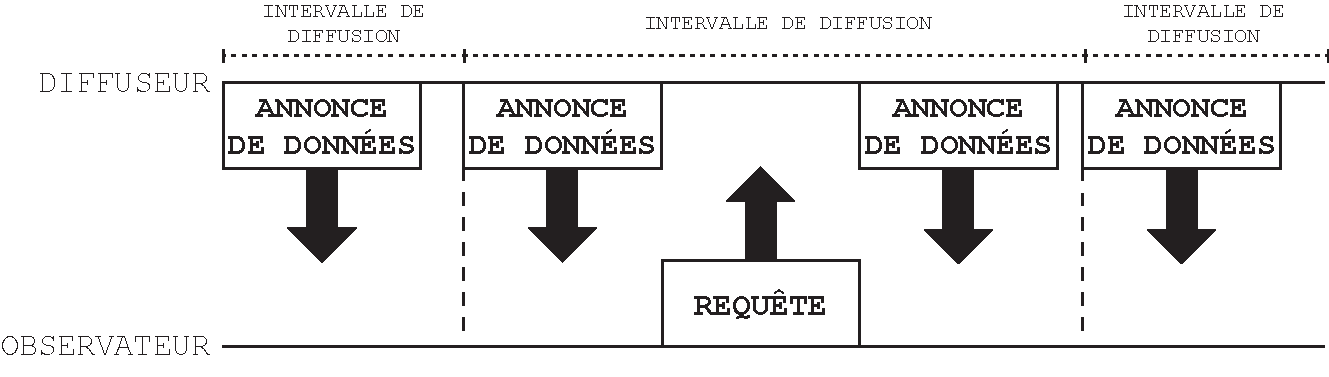
\includegraphics[width=.85\linewidth]{chapter3/ble_broadcast_process.pdf}
		\label{fig:ble_broadcast_process}
    }
    \\[10pt]
	\subfloat[Échange de données en mode connexion]{
		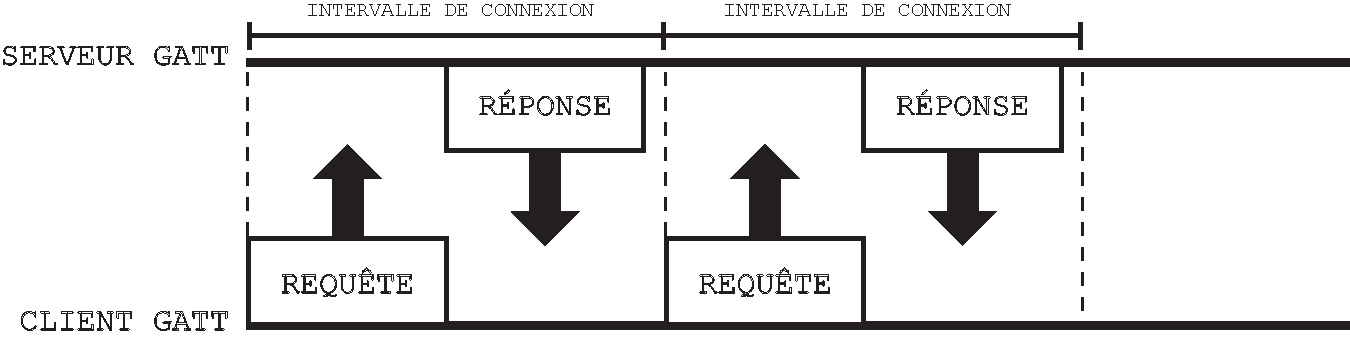
\includegraphics[width=.85\linewidth]{chapter3/ble_connect_process.pdf}
		\label{fig:ble_connect_process}
	}
	\caption{Illustration du processus d'échange de données dans les deux modes de fonctionnement du \acs{BLE}, soit les modes diffusion et connexion.}
\end{figure}

\subsection{Les Services Web}

Les services web permettent à différentes applications de communiquer entre elles en fournissant une plateforme commune pour l'échange de données. Les requêtes et les réponses émises par les applications sont soumises à des standards. Parmi les plus populaires, il est possible de retrouver le protocole \ac{SOAP}, l'architecture \acl{REST} (\acs{REST}) et le protocole \acl{COAP} (\acs{COAP}).

\subsubsection{Le protocole \ac{SOAP}}

Le protocole \ac{SOAP}, tout comme le modèle \textit{publish/subscribe}, est lui aussi utilisé dans les habitats intelligents depuis leur apparition. En effet, c'est principalement le cas de ceux ayant opté pour une architecture par composants et plus particulièrement \ac{OSGi} (comme Gator-tech \citep{Helal2005}), puisque cette technologie repose sur \ac{SOAP} pour tirer profit des services web. Depuis, de nombreux travaux se sont intéressés à l'interopérabilité des données ambiantes fournies par les habitats intelligents avec les données produites par les \textit{wearable devices} \citep{Perumal2008, Cubo2014, Diaz-Rodriguez2018}.

\ac{SOAP} est un protocole d'échange d'information structuré qui repose sur le langage \ac{XML}. Bien que ce dernier puisse être utilisé au-dessus de plusieurs autres protocoles tels que \ac{SMTP}, \ac{TCP} ou \ac{UDP}, il est majoritairement employé comme couche supérieure à \acl{HTTP} (\acs{HTTP}). Le protocole \ac{SOAP} appartient au modèle client/serveur et permet aussi bien l'appel de procédures respectant les propriétés ACID (Atomicité, Cohérence, Isolation et Durabilité), que le transfert d'informations. Dans ce dernier cas, un message est envoyé au serveur qui va alors traiter l'information et répondre au client.

Un message \ac{SOAP} est un document \ac{XML} qui contient un en-tête (\textit{header}) ainsi qu'un corps (\textit{body}), le tout encapsulé dans une enveloppe. Cette dernière indique que le document XML correspond à un message \ac{SOAP} et identifie le début ainsi que la fin de du message. L'en-tête, qui demeure facultatif, peut contenir différents attributs relatifs au message. Le corps, quant à lui obligatoire, contient les informations soit de la requête faite par le client, soit de la réponse du serveur, ainsi que des informations à propos des erreurs qui pourraient survenir. Les informations contenues dans le corps du message \ac{SOAP} sont organisées sous forme de blocs. La figure \ref{fig:soap_msg} montre un exemple d'échange de messages \ac{SOAP} à travers \ac{HTTP} qui permet d'obtenir la valeur du capteur cardiaque d'un dispositif quelconque.

\begin{figure}[b!]
    \centering
	\subfloat[Requête \acs{SOAP}]{
		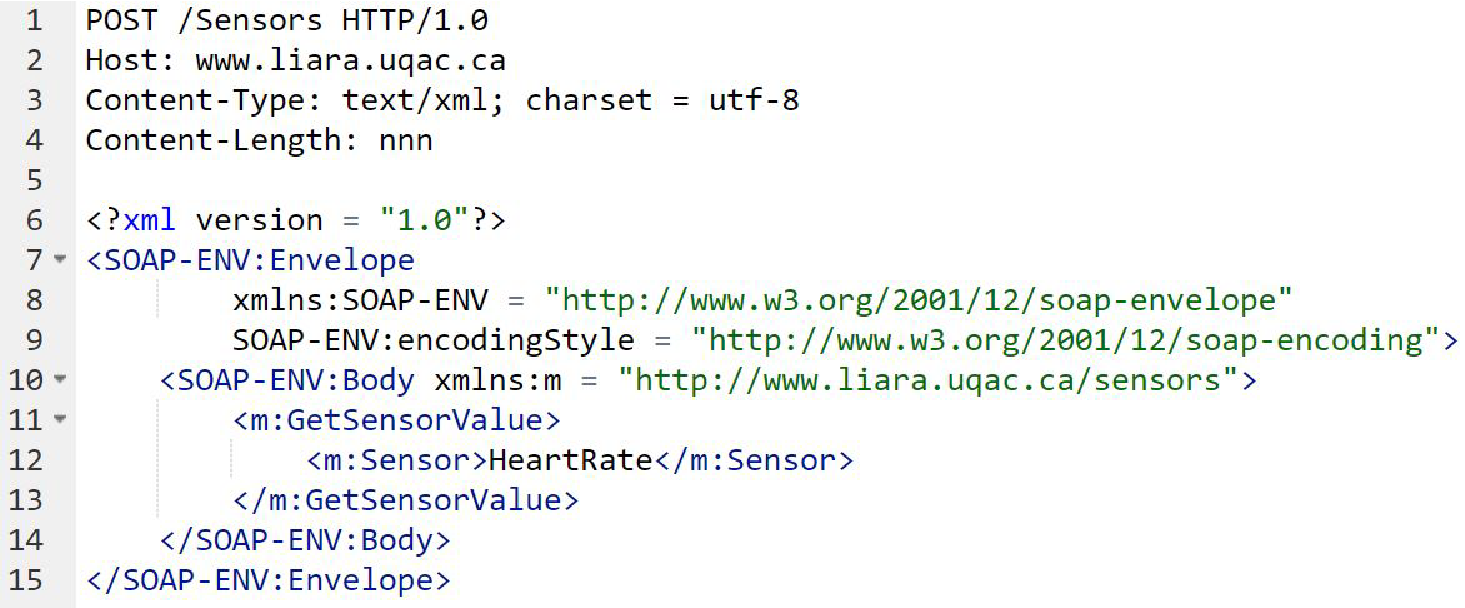
\includegraphics[width=.85\linewidth]{chapter3/soap_req.pdf}
		\label{fig:soap_req}
    }
    \\[20pt]
	\subfloat[Réponse \acs{SOAP}]{
		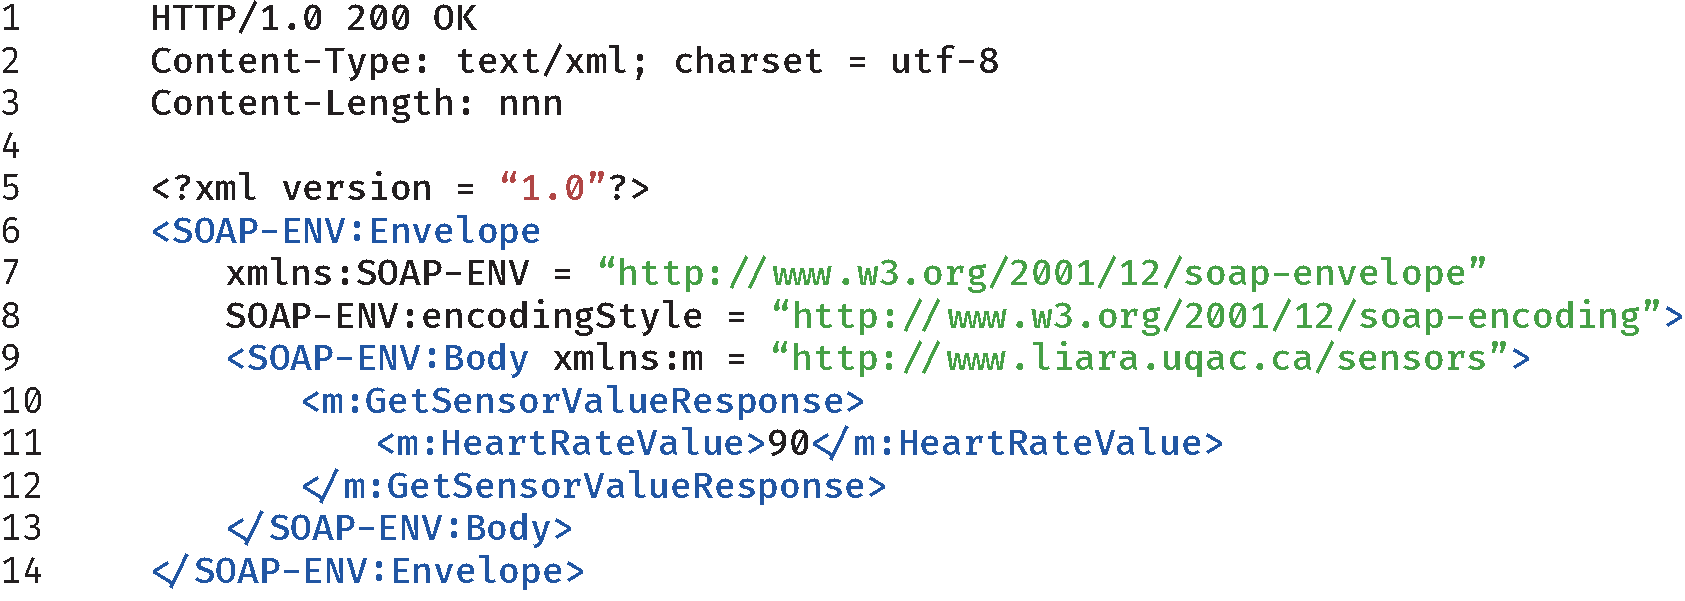
\includegraphics[width=.85\linewidth]{chapter3/soap_res.pdf}
		\label{fig:soap_res}
    }
    \caption{Exemple d'un échange de messages \acs{SOAP} entre un client et un serveur pour obtenir la valeur du capteur cardiaque.}
    \label{fig:soap_msg}
\end{figure}

L'avantage principal de l'utilisation de \ac{SOAP} comme méthode de communication est principalement la sécurité qu'offre ce protocole. En effet, ce dernier peut être implémenté par dessus une couche de chiffrement \ac{SSL}, mais il permet également d'exploiter la spécification \textit{Web Services Security ou WS-Security} qui apporte des fonctionnalités de sécurité supplémentaires appréciées des entreprises. Cependant, il demeure un protocole peu flexible et relativement lourd et complexe à mettre en place.

\subsubsection{L'architecture \ac{REST}}

Dès le début des années 2000, l'introduction des architectures de type \ac{REST} \citep{Fielding2000} a permis de remplacer petit à petit le protocole \ac{SOAP}, venant ainsi combler certaines de ses lacunes. Le principal avantage de ces architectures est leur indépendance vis-à-vis des protocoles existants. En effet, bien que les architectures \ac{REST} soient aussi majoritairement définies par-dessus \ac{HTTP}, elles pourraient tout autant l'être sur n'importe quel autre protocole\textemdash tant que celui-ci admet un schéma d'\ac{URI} normalisé. Tout comme pour \ac{SOAP}, les architectures \ac{REST} s'appuient sur le modèle de communication client/serveur. Cependant, à l'inverse de \ac{SOAP}, un service web \ac{REST} est sans état, c'est-à-dire que le serveur ne connaît pas l'état de chaque client entre les requêtes qu'il doit traiter. Ainsi, du point de vue du serveur, chaque requête est une entité distincte des autres. De plus, contrairement à \ac{SOAP}, qui impose le format d'échange de données en \ac{XML}, \ac{REST} accepte que les ressources, c'est-à-dire, les données échangées entre le client et le serveur, soient exprimées selon plusieurs formats de données tels que \ac{XML}, \ac{JSON} ou encore \ac{HTML}. Ceci garantit alors un meilleur support pour les clients.

Lorsqu'elle est définie sur \ac{HTTP}, une architecture \ac{REST} manipule ses ressources avec les différentes méthodes \ac{HTTP} (\texttt{GET}, \texttt{POST}, \texttt{PUT}, \texttt{DELETE}, \texttt{PATCH}). Ainsi, lorsqu'un client émet une requête indiquant l'opération qu'il souhaite effectuer sur une ressource donnée, la réponse transmise par le serveur contient alors deux éléments importants—l'en-tête et le corps de la réponse. Plus précisement, l'en-tête contient des informations importantes à propos de l’échange d’information :

\begin{itemize}[label=\textbullet]
    \item
        La version du protocole \ac{HTTP} utilisé pour le transport des données.
    \item
        Le code \ac{HTTP} \citep{Fielding2014} qui indique l'état de la réponse.
    \item
        Le format de donnée.
    \item
        \textit{etc.}
\end{itemize}

\noindent Le corps de la réponse, quant à lui, peut contenir une ressource, un message d'erreur, \textit{etc.} La figure \ref{fig:rest_get} illustre le processus de communication entre un client et un serveur dans une architecture \ac{REST} basée sur les méthodes \ac{HTTP}. Le client demande l'obtention de la valeur du capteur cardiaque d'un dispositif quelconque. Cette ressource est identifiée par l'\ac{URI} : \texttt{http://liara.uqac.ca/sensors/health/1}. Puisque le serveur est capable de fournir la réponse attendue, et ce, sans erreur, le code \ac{HTTP} 200, ainsi que le nom et la valeur du capteur sont renvoyés au client au format \ac{JSON}, tel que précisé dans l'en-tête de la réponse.

\begin{figure}[H]
	\centering
	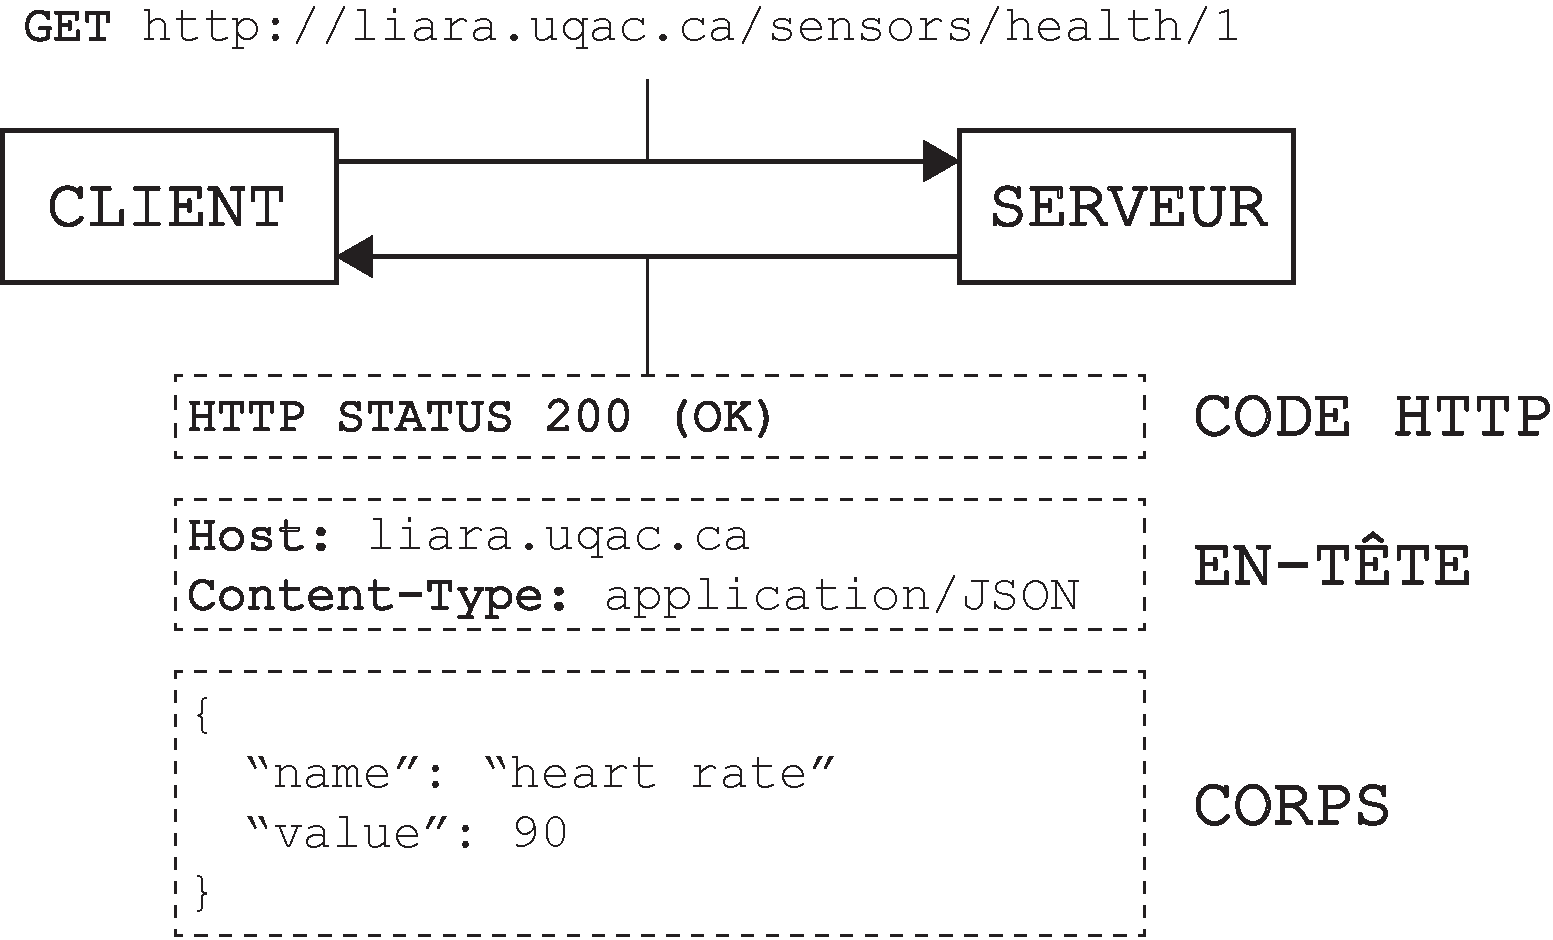
\includegraphics[width=10cm]{chapter3/rest_get.pdf}
        \caption{Illustration d'un échange de messages entre un client et un serveur dans une architecture \ac{REST} basée sur \ac{HTTP} qui permet de récupérer la valeur d'un capteur cardiaque.}
	\label{fig:rest_get}
\end{figure}

\subsubsection{Le protocole \ac{COAP}}

Plus récemment, la recrudescence du nombre d'objets connectés et plus particulièrement de \textit{wearable devices} a fait émerger plusieurs problématiques inhérentes à la limitation de leurs ressources telles qu'une puissance de calcul restreinte, une faible quantité de mémoire ou encore une autonomie réduite. Cependant, la limitation de ces dispositifs implique également de nouvelles problématiques au regard du processus d'échange de données. En effet, malgré une meilleure efficacité qu'avec le protocole \ac{SOAP}, tant en termes de débit qu'en termes de consommation de ressources, l'exploitation des services web à travers une architecture \ac{REST} s'est parfois montrée inadaptée dans le contexte de l'\acs{IoT} \citep{Kovatsch2011}. En effet, lorsqu'une architecture \ac{REST} repose sur le protocole \ac{HTTP}, il a été observé qu'une grande fréquence de requêtes ne retournant qu'un nombre faible de données entraînait une surcharge réseau, principalement à cause des en-têtes \ac{HTTP} qui sont encodés en \ac{ASCII} \citep{Shelby2010}. Néanmoins ce cas de figure correspond au fonctionnement typique d'un réseau de capteurs sans-fil, où chaque message qui est envoyé correspond généralement à une seule mesure. Par conséquent, le protocole \ac{COAP} a été introduit par \cite{Shelby2014} afin de mieux répondre aux besoins des appareils ayant de fortes contraintes liées au débit, à la consommation et à la puissance de calcul. Malgré son jeune âge, plusieurs recherches se sont tournées vers une implantation de \ac{COAP} au sein des habitats intelligents \citep{Bergmann2012, Mainetti2015}. Par ailleurs, de récents travaux, comme celui introduit par \cite{Plantevin2017}, ont proposé de nouveaux protocoles de communication qui s'inspirent de la spécification de \ac{COAP}. Bien qu'ils soient encore très peu exploités, ceux-ci visent principalement à mieux intégrer l'\acs{IoT} au sein des habitats intelligents, puisqu'ils permettent d'optimiser davantage le processus d'échange de données.

Pour mettre en place une architecture \ac{REST}, \ac{COAP} reprend plusieurs concepts de \ac{HTTP} comme les échanges de messages asynchrones, par exemple. Cependant plusieurs optimisations ont été faites pour le rendre plus adapté aux systèmes embarqués tel que la nécessité d'utiliser le protocole \ac{UDP} qui permet de se passer des mécanismes de fiabilité qui sont obligatoire avec le protocole \acs{TCP} lors d'échanges de messages. En outre, les en-têtes sont compressés afin de réduire la complexité du décodage et les besoins en bande passante. Les messages \ac{COAP} contiennent les informations suivantes :

\begin{itemize}[label=\textbullet]
    \item
        La version du protocole utilisée pour le transport des données.
    \item
        Le type du message indique s'il s'agit, d'un message fiable qui exige un acquittement (\texttt{CON}), d'un message asynchrone qui n’a pas besoin d’être acquitté (\texttt{NON}), d'un message d’acquittement, c'est-à-dire, une réponse à une requête \texttt{CON} (\texttt{ACK}), d'un message qui indique que le serveur a bien reçu la requête, mais qu'il n’a pas le contexte nécessaire pour fournir une réponse (\texttt{RST}).
    \item
        Le nombre d'options transmises dans l'en-tête (\texttt{OC}).
    \item
        Un code qui indique si le message est une requête, une réponse ou un message vide. Dans le cas d’une requête, la méthode utilisée est également précisée. Elles sont identiques aux méthodes \ac{HTTP}.
    \item
        Un identifiant unique pour détecter les messages dupliqués et pour faire la correspondance entre un message \texttt{CON} et son \texttt{ACK} respectif.
    \item
        Différentes options, par exemple, un paramètre pour définir la durée de validité des données transmises.
    \item
        Les données en elles-mêmes.
\end{itemize}

\noindent La figure \ref{fig:coap_get} illustre le processus de communication entre un client et un serveur dans une architecture \ac{REST} basée sur \ac{COAP}. Le client demande l'obtention de la valeur du capteur cardiaque d'un dispositif quelconque où la requête et la ressource sont respectivement identifiées par le code \texttt{0x4d45} et l'\ac{URI} \texttt{/sensors/health/hr}. Le serveur transmet alors immédiatement le message \texttt{ACK} ainsi que la valeur du capteur.

\begin{figure}[H]
	\centering
	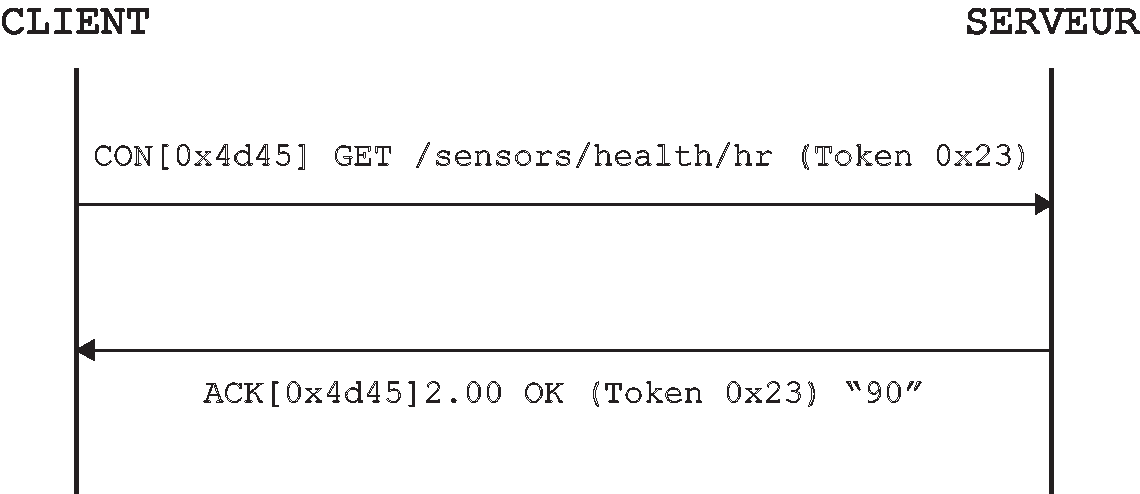
\includegraphics[width=10cm]{chapter3/coap_get.pdf}
        \caption{Illustration d'un échange de messages entre un client et un serveur dans une architecture \ac{REST} basée sur \ac{COAP} qui permet de récupérer la valeur d'un capteur cardiaque.}
	\label{fig:coap_get}
\end{figure}

Puisque la différence majeure entre \ac{COAP} et \ac{HTTP} réside dans l'utilisation du protocole \ac{UDP}, sous-jacent, ceci lui permet de supporter le \textit{multicast}. Aussi, comme \ac{COAP} est principalement conçu pour l'\acs{IoT}, ce protocole se base principalement sur IPv6 bien que, dans de plus rare cas, il puisse également exploiter IPv4. La communication à travers IPv6 permet donc à ce protocole de mieux prendre en compte le volume d'entités qui composent un réseau de capteurs sans-fil. Enfin, il permet de mettre en place aussi bien un modèle client/serveur, tel qu'illustré dans l'exemple précédent, qu'un modèle \textit{publish/subscribe} à l'instar du protocole \ac{MQTT}.

\section{Conclusion}

Dans un premier temps, ce chapitre s'est intéressé à la couche matérielle qui compose les \textit{wearable devices}. Les capteurs les plus adéquats pour être embarqués dans ce type de dispositifs ont été regroupés en différentes catégories qui sont : les capteurs de mouvement, les capteurs physiologiques, les capteurs de courbure et de force ainsi que les capteurs environnementaux. Bien qu'il en existe beaucoup d'autres, ce chapitre a montré que ceux-ci demeurent les plus utilisés dans divers domaines de recherche tels que la réhabilitation, la surveillance de la santé et surtout dans la reconnaissance de gestes et d'activités.

Ensuite, ce chapitre a présenté les technologies de communication sans-fil actuellement employées par les \textit{wearable devices}, mais également les futures évolutions de chacune d'elles. Il est apparu que toutes s'inscrivent dans l'optique de mieux prendre en compte le nombre grandissant d'objets connectés, plus particulièrement en ce qui concerne leur limitation énergétique. De plus, en ne considérant que les capacités actuelles de chaque technologie, ce chapitre a proposé un comparatif de leurs différences en termes de capacité de portée, débit et robustesse. Ceci a permis de conclure que le choix de la technologie à adopter dans le processus de conception de \textit{wearable devices} doit se faire en fonction des contraintes liées à leur utilisation.

Enfin, dans sa dernière partie, ce troisième chapitre a exposé les différents protocoles et architecture de haut niveau permettant aux \textit{wearable devices} d'échanger leurs données avec d'autres entités qui composent un réseau (capteurs intelligents, serveur central, \textit{etc.}). Ainsi, dans les travaux sur les habitats intelligents et leurs évolutions pour y intégrer l'\acs{IoT}, deux principaux modèles pour l'échange de données ont été retenus. Le premier est le modèle \textit{publish/subscribe} et plus particulièrement le protocole \acs{MQTT}. Le second concerne le modèle client/serveur, plus traditionnel. Bien qu'il admette un fonctionnement particulier, le cas du \acs{BLE} s'appuie fortement sur ce deuxième modèle. De plus, des méthodes plus récentes issues du web social, comme la consommation de services web, appartiennent également à un modèle client/serveur. Pour tirer profit des services web, plusieurs technologies comme le protocole \acs{SOAP} ou les architectures \acs{REST} ont été mises en place au sein des infrastructures d'habitats intelligents. Cependant, certaines limitations quant à l'intégration de l'\acs{IoT} ont pu être observées. Pour combler ces problématiques, de nouvelles implémentations comme le protocole \acs{COAP} ont été mises en place dans ces habitats.